\section{Clinical Action Assurance Framework}
\subsection{Purpose and trust boundary}
CAA is a proposed reference framework for connecting clinical evidence, institutional authority, bounded execution, and verified effects. It draws on lifecycle governance and risk-management principles \cite{who2024,nist2023,nist2024,governingagents2023}, as well as interoperable authorization and provenance mechanisms \cite{smart2024,fhir2019}. These sources do not certify an agent's clinical safety. CAA makes explicit the software and clinical assumptions needed to operationalize them.

Figure~\ref{fig:caa} places policy and identity outside the planner. An institutionally trusted context supplies the initiating principal, purpose, patient, encounter, policy version, permitted operations, and required reviewer. The planner can propose typed actions based on an evidence workspace; it cannot mint its own permissions or clinician approval. An admission gate evaluates the proposal against current context and evidence. Only an admitted contract reaches a bounded adapter. A destination receipt and post-state check then determine whether the intended effect occurred. Audit, monitoring, escalation, suspension, and domain-specific recovery span the process.

\begin{figure*}[t]\centering
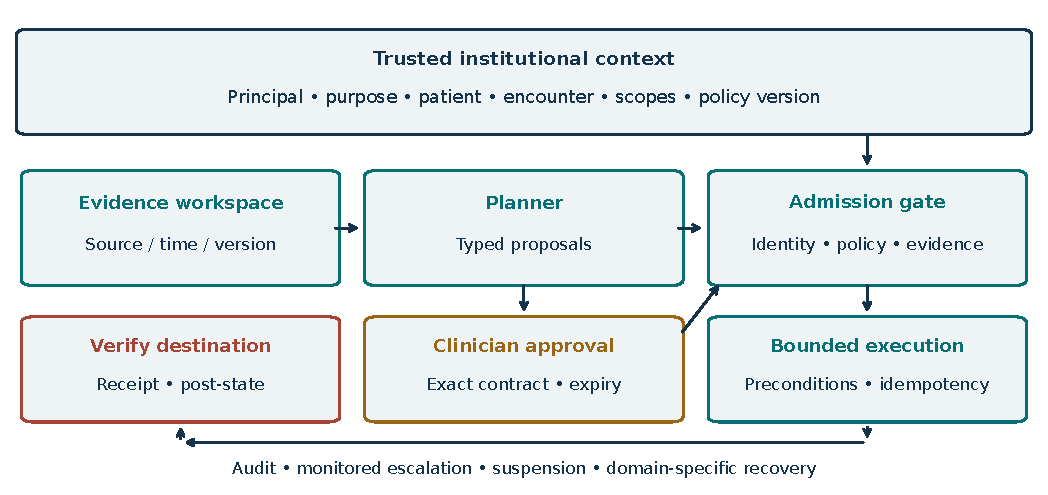
\includegraphics[width=\textwidth]{figures/fig3_caa_framework.pdf}
\caption{Proposed Clinical Action Assurance architecture. Trusted institutional identity and policy constrain the planner; exact-contract approval and current-state checks precede bounded execution. Destination verification and monitored escalation follow execution. The diagram is a proposed design, not a clinically validated system.}\label{fig:caa}
\end{figure*}

\subsection{Action contract and admission semantics}
A minimal action contract can be represented as
\begin{equation}
\kappa=(u,e,\mathrm{op},\mathbf{x},\mathbf{v},\mathcal{E},[t_0,t_1],\alpha,k),
\end{equation}
where $u$ and $e$ bind patient and encounter; $\mathrm{op}$ and $\mathbf{x}$ identify a typed operation and its arguments; $\mathbf{v}$ specifies required resource versions; $\mathcal{E}$ identifies supporting evidence; $[t_0,t_1]$ is the validity interval; $\alpha$ identifies approval; and $k$ is an idempotency key. The principal, purpose, and policy version must be bound in the contract or in trusted context used to validate it. Approval should refer to canonical contract content excluding the approval token itself, avoiding circular digest construction.

For policy $\theta$, let
\begin{equation}
G_\theta(\kappa)=I\wedge S\wedge V\wedge P\wedge E\wedge A\wedge L,
\end{equation}
where $I$ checks identity/encounter binding, $S$ allowed scope, $V$ current resource preconditions, $P$ domain constraints, $E$ evidence admissibility/freshness, $A$ approval, and $L$ temporal and operational limits. Each obligation should be true, false, or unresolved. A false obligation denies execution; an unresolved obligation defers it for resolution. Absence of a check is not permission. This conjunction is a control specification, not a probabilistic safety guarantee. In particular, domain-rule completeness and clinical evidence correctness are assumptions that need independent assessment.

\subsection{Approval and execution}
A clinician should review the actual proposed effect, its evidence, current patient context, and alternatives. Approval must be bound to the exact canonical payload, resource versions, and relevant policy. Mutation after approval invalidates that approval. A digest detects content change but does not authenticate the reviewer; production systems require genuine identity, authorization, secure token handling, and appropriate nonrepudiation controls.

The adapter should expose the minimum permitted operation set and reject requests that attempt to bypass preconditions. Execution should atomically enforce the destination state version wherever the underlying system allows it. A request key must map to one exact payload: repeated identical requests can return an established receipt, but changed content with the same key must fail. Revoked permissions or changed policy should remain effective even during retry handling. Technical success must be followed by checks of patient, operation, destination effect, and relevant state. A mismatch after commitment triggers reconciliation and escalation; it cannot retroactively make the effect disappear.

\subsection{Worked illustrative workflow}
Consider creation of a follow-up review task from a synthetic observation. The planner proposes a typed task for SYNTHETIC-P001 in SYNTHETIC-E001, referencing observation version 3. Trusted context permits only that task type and identifies an authorized reviewer. A clinician approval binds the proposal digest and expiry. If the observation changes to version 4 before commitment, the adapter rejects the stale precondition and requests a new review. If the write commits but its network response is lost, a retry with the same payload/key retrieves the established receipt. If the destination reports another patient or an unexpected task, the system escalates the unknown or mismatched effect.

The accompanying in-memory implementation illustrates these software obligations. It uses synthetic identifiers, a single task operation, explicit state versions, approval digests, an idempotency registry, and receipt checks. It has no LLM, live EHR, authenticated clinical identity, or clinically validated rule set. Its negative and retry tests are software invariant tests, not evidence that autonomous care is safe. This narrow example is intentionally reviewable: it demonstrates what must be specified before a richer agent architecture can be assessed.

\subsection{Monitoring and recovery ownership}
Monitoring must detect both unexpected writes and expected effects that never occur. Every deferred or escalated item needs a receiving role, acknowledgement, deadline, and overdue response. An institution should define suspension criteria, version-change review, and domain-specific recovery. Audit records should preserve source/evidence identifiers, policy and model versions, proposed and executed payloads, approval identity, receipts, and relevant post-state. Detailed reasoning traces may expose sensitive data or provide misleading rationales; operational audit should prioritize necessary observable evidence and apply governance to its retention.
